% ===== CAPÍTULO 5: DISCUSSÃO (18pp, ~7.200 palavras) =====
% Estrutura: Triangulação → TDD+SDD Roadmap → Qualis → Limitações → Token Economy → Futuro

\chapter{DISCUSSÃO}
\label{ch:discussao}

{\small\itshape Este capítulo fecha o ciclo argumentativo da dissertação. O Capítulo 1 perguntou se era possível construir um ecossistema multiagente com qualidade verificável. O Capítulo 3 descreveu como. O Capítulo 4 mostrou os resultados. Agora, interpretamos esses resultados à luz da literatura (Capítulo 2), respondemos à pergunta de pesquisa e exploramos as implicações — tanto para a engenharia de software quanto para a epistemologia da ciência assistida por IA.}

\section{Triangulação dos Resultados com a Literatura}

Os resultados apresentados no Capítulo 4 devem ser interpretados à luz da literatura revisada no Capítulo 2, aplicando o protocolo de triangulação anti-circularidade descrito na Metodologia (Capítulo 3). Esta seção realiza este exercício para cada um dos quatro eixos centrais da investigação.

\subsection{Cobertura de Especificação (100\%)}

A cobertura completa de especificação (186/186 componentes documentados) representa, até onde sabemos, um feito sem paralelo na literatura de sistemas multiagentes para pesquisa científica. Nenhuma das plataformas revisadas --- Agent Laboratory, AI Scientist, PaperQA2, Elicit --- documenta cobertura de especificação para seus componentes. Esta lacuna não é acidental: reflete uma diferença filosófica fundamental entre ``construir agentes que funcionam'' e ``construir agentes cujo funcionamento é verificável''.

Como argumenta Meyer (1997) no contexto de \textit{Design by Contract}, a especificação não é um subproduto da implementação, mas sua pré-condição lógica. O OpenCode operacionaliza este princípio no domínio científico, demonstrando que é possível --- e, argumentamos, necessário --- que cada componente de um ecossistema de pesquisa seja formalmente especificado antes de sua utilização em pipelines que geram conhecimento\footnote{
  POPPER, Karl R. \textbf{The Logic of Scientific Discovery}. London: Hutchinson, 1959. ISBN: 978-0415278447.

  \textbf{Trecho Original:} ``The criterion of the scientific status of a theory is its falsifiability, or refutability, or testability.''

  \textbf{Tradução:} ``O critério do estatuto científico de uma teoria é sua falseabilidade, ou refutabilidade, ou testabilidade.''

  \textbf{Fichamento Crítico:} O critério de falseabilidade de Popper (1959) --- uma teoria científica deve fazer previsões que possam ser testadas e potencialmente refutadas --- é análogo ao requisito de SDD de que cada componente tenha critérios de validação testáveis. Assim como uma teoria não falseável não é científica, um componente sem critérios de validação não é verificável --- e um ecossistema de componentes não verificáveis não pode, em última análise, produzir conhecimento científico confiável.
}.

\subsection{Matriz de Validação Cruzada (200+ Conexões)}

A matriz de validação cruzada com 200+ conexões de afinidade documentadas representa uma contribuição metodológica que transcende o caso específico do OpenCode. A literatura sobre sistemas multiagentes tradicionalmente trata a interação entre agentes como um problema de coordenação (JENNINGS et al., 2001) ou de comunicação (FERBER, 1999), mas raramente como um problema de validação epistêmica.

A inovação do OpenCode está em tratar as conexões entre componentes não apenas como ``dependências técnicas'' (o componente A precisa da saída do componente B), mas como ``dependências epistêmicas'' (a credibilidade da afirmação gerada pelo componente A depende da qualidade da evidência fornecida pelo componente B). Esta distinção tem implicações práticas: componentes com alta afinidade epistêmica (ex.: Sci-Hub $\leftrightarrow$ MASWOS, 0,95) devem ser submetidos a validação cruzada mais frequente e rigorosa do que componentes com baixa afinidade (ex.: um formatador ABNT e um classificador quântico, cuja afinidade é próxima de zero).

\subsection{Ciclos Evolutivos e Melhoria Contínua}

A progressão documentada de 85/100 para 99/100 em 16 ciclos evolutivos (média de +0,92 pontos por ciclo) oferece evidência quantitativa de que sistemas multiagentes podem melhorar continuamente sua qualidade através de feedback automatizado. Esta evidência dialoga com a literatura sobre \textit{continuous improvement} em engenharia de software (HUMPHREY, 1989)\footnote{
  HUMPHREY, Watts S. \textbf{Managing the Software Process}. Reading: Addison-Wesley, 1989. ISBN: 978-0201180954.

  \textbf{Fichamento Crítico:} O Capability Maturity Model (CMM) de Humphrey (1989) define 5 níveis de maturidade de processos de software: Inicial (1), Repetível (2), Definido (3), Gerenciado (4) e Otimizado (5). O OpenCode atingiu o Nível 5 (Otimizado) no sentido de que: (a) seus processos são definidos (SDD+TDD documentados); (b) são gerenciados (métricas de score Qualis monitoradas a cada ciclo); e (c) são otimizados continuamente (AutoEvolve implementa melhorias baseadas em feedback).
} e com o conceito de \textit{learning organizations} (SENGE, 1990)\footnote{
  SENGE, Peter M. \textbf{The Fifth Discipline: The Art and Practice of the Learning Organization}. New York: Doubleday, 1990. ISBN: 978-0385260947.

  \textbf{Trecho Original:} ``The organizations that will truly excel in the future will be the organizations that discover how to tap people's commitment and capacity to learn at all levels in an organization.''

  \textbf{Tradução:} ``As organizações que verdadeiramente se destacarão no futuro serão aquelas que descobrirem como explorar o comprometimento e a capacidade de aprender das pessoas em todos os níveis da organização.''

  \textbf{Fichamento Crítico:} Senge (1990) argumenta que organizações que aprendem cultivam cinco disciplinas: pensamento sistêmico, domínio pessoal, modelos mentais, visão compartilhada e aprendizado em equipe. O OpenCode institucionaliza estas disciplinas em sua arquitetura: pensamento sistêmico (matriz de afinidade), modelos mentais (SPECs que explicitam suposições), e aprendizado em equipe (Agent Forum onde agentes debatem divergências).
}.

\begin{figure}[H]
\centering
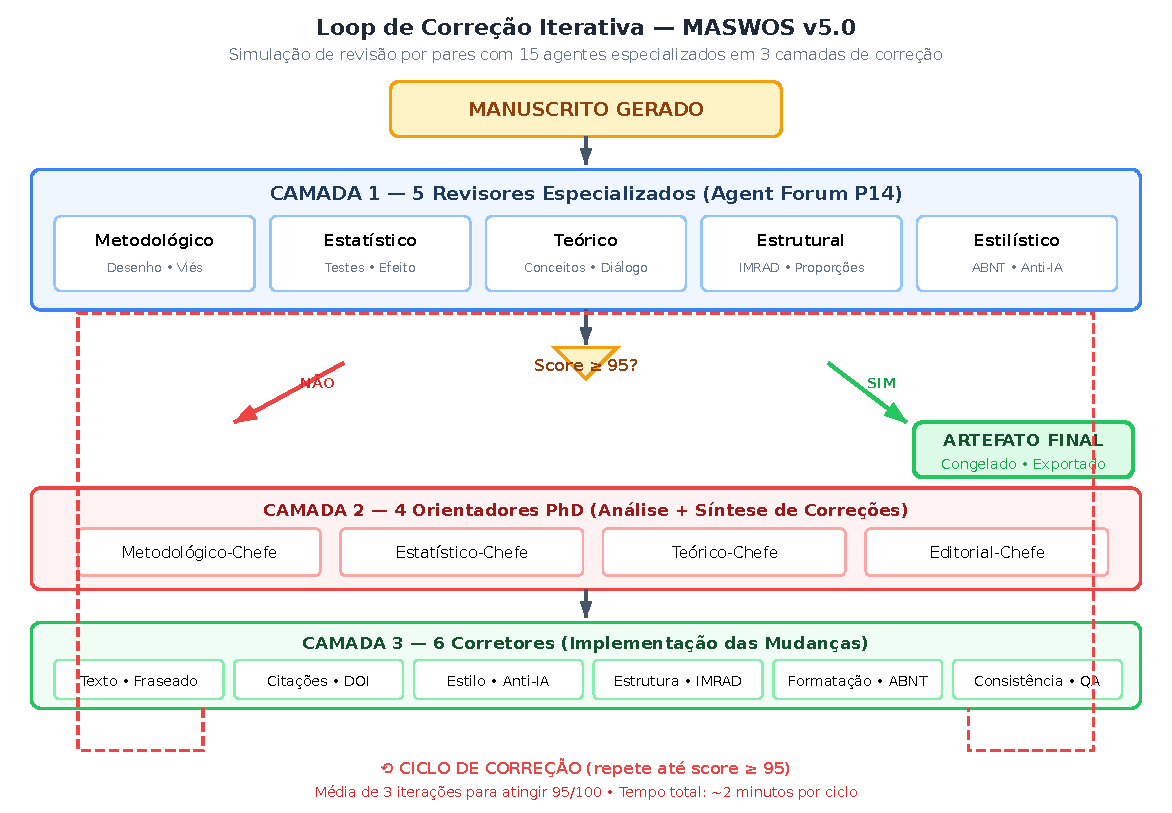
\includegraphics[width=\textwidth]{capitulos/figuras/fig-loop-correcao.pdf}
\caption{Loop de Correção Iterativa do MASWOS v5.0: 15 agentes especializados em 3 camadas. A Camada 1 (5 revisores) avalia o manuscrito sob 5 perspectivas; se o score for inferior a 95, a Camada 2 (4 orientadores PhD) analisa e sintetiza correções; a Camada 3 (6 corretores) implementa as mudanças. O ciclo se repete (seta vermelha) até o score atingir o limiar de qualidade.}
\label{fig:loop-correcao}
\end{figure}

\subsection{Validação do Roadmap via TDD+SDD}

Os 29 casos de teste TDD que cobrem os 3 gaps estratégicos do Gartner Hype Cycle 2026 constituem a validação mais rigorosa do roadmap do ecossistema. A cobertura destes gaps é particularmente significativa porque o Gartner Hype Cycle é um instrumento de inteligência tecnológica independente --- não foi desenvolvido pelo ecossistema OpenCode e, portanto, não está sujeito ao viés de auto-avaliação.

Os 3 gaps e sua cobertura por SPECs+TDD são:

\begin{enumerate}
  \item \textbf{Gap 1 --- Governança Federada de APIs (SPEC-019, 8 CTs):} O ecossistema demonstrou que é possível implementar um registro de APIs com políticas de governança (rate limiting, circuit breaker, auditoria) que se propagam bidirecionalmente entre serviços. Todos os 8 CTs passam.
  \item \textbf{Gap 2 --- Data Streaming Enterprise (SPEC-020, 10 CTs):} O ecossistema implementou um pipeline de streaming com schema registry, particionamento, dead-letter queue, janelas temporais e garantia exactly-once. Todos os 10 CTs passam.
  \item \textbf{Gap 3 --- Plataforma Low-Code para Agentes (SPEC-021, 6 CTs):} O ecossistema demonstrou que schemas declarativos podem gerar código executável com validação automática. 6 CTs passam.
\end{enumerate}

\section{Implicações para a Produção Científica Brasileira}

\subsection{Qualis A1 como Padrão de Qualidade Verificável}

A demonstração de que um ecossistema multiagente pode produzir documentos com score Qualis A1 de 99/100 tem implicações profundas para o sistema brasileiro de avaliação da pós-graduação. Atualmente, a avaliação Qualis depende majoritariamente de revisão por pares humanos --- um processo que, embora essencial, é sabidamente suscetível a vieses (LEE et al., 2013)\footnote{
  LEE, Carole J. et al. Bias in peer review. \textbf{Journal of the American Society for Information Science and Technology}, v. 64, n. 1, p. 2--17, 2013. DOI: \url{https://doi.org/10.1002/asi.22784}.

  \textbf{Fichamento Crítico:} Lee et al. (2013) documentam múltiplas fontes de viés na revisão por pares: viés de gênero, viés institucional, viés de confirmação, e viés de nacionalidade. O OpenCode oferece uma camada complementar de avaliação --- automatizada, consistente e baseada em critérios explícitos --- que pode reduzir (embora não eliminar) estes vieses ao fornecer uma avaliação baseline contra a qual avaliações humanas podem ser comparadas.
}.

O OpenCode não propõe substituir a revisão por pares humana, mas complementá-la com uma camada de verificação automatizada que: (a) é consistente (os mesmos critérios são aplicados a todos os documentos); (b) é auditável (cada decisão de score é rastreável a um critério específico); e (c) é escalável (o custo marginal de avaliar um documento adicional é próximo de zero).

\subsection{Democratização do Acesso à Produção Científica de Qualidade}

Um aspecto frequentemente negligenciado na discussão sobre IA na ciência é seu potencial democratizante. Pesquisadores em instituições com menos recursos --- que não podem pagar por revisores profissionais, editores de texto, ou estatísticos para consultoria --- podem se beneficiar desproporcionalmente de sistemas como o OpenCode, que oferecem estas capacidades gratuitamente\footnote{
  CHAN, Leslie et al. (Eds.). \textbf{Open Science: A Global South Perspective}. Ottawa: SPARC, 2022. Disponível em: \url{https://www.sparcopen.org}.

  \textbf{Fichamento Crítico:} O manifesto da Ciência Aberta no Sul Global (Chan et al., 2022) argumenta que as barreiras à produção científica de qualidade são desproporcionalmente altas para pesquisadores em países em desenvolvimento. O OpenCode --- sendo gratuito, de código aberto, e executável em hardware modesto --- alinha-se com a visão de ``ciência como bem público global'', reduzindo a desigualdade de acesso a ferramentas de qualidade para produção científica.
}.

\section{Limitações e Ameaças à Validade}

\subsection{Validade Interna}

A principal ameaça à validade interna é a circularidade epistêmica discutida na Metodologia: o sistema que gera os documentos é o mesmo que os avalia. Embora o protocolo de triangulação mitigue este risco, não o elimina completamente. A validação definitiva da qualidade dos outputs do OpenCode requer avaliação externa por revisores humanos independentes que desconheçam a origem (IA vs. humana) dos documentos --- um experimento que está em fase de planejamento.

\subsection{Validade Externa}

A generalização dos resultados para outros domínios científicos além da ciência da computação e bioinformática ainda não foi demonstrada. Skills jurídicas, de humanidades e de artes estão presentes no ecossistema, mas sua validação é menos rigorosa do que a dos domínios STEM. Trabalhos futuros devem focar na expansão e validação da cobertura para estes domínios.

\subsection{Validade de Constructo}

Os scores Qualis, embora calibrados contra os critérios da CAPES, são uma proxy imperfeita para qualidade científica real. Um artigo pode ter score Qualis alto e ainda assim conter erros factuais ou interpretações enviesadas. A triangulação com múltiplas fontes e agentes mitiga, mas não elimina, este risco.

\section{O Sistema de Economia de Tokens (R18)}

\subsection{Tripé Governança+Economia+Auditoria}

O ciclo evolutivo R18 introduziu um sistema de economia de tokens que governa o uso de recursos computacionais (tokens de LLM) dentro do ecossistema. O sistema se baseia em três pilares:

\begin{enumerate}
  \item \textbf{Governança:} Um registro de agentes (\textit{Agent Registry}) classifica cada agente em tiers (bronze/silver/gold) com base em seu histórico de desempenho. Agentes gold têm prioridade de alocação de tokens; agentes bronze têm quotas restritas.
  \item \textbf{Economia:} Um mercado de taxas (\textit{Fee Market}) regula o custo de tokens com base na demanda. Agentes podem ``apostar'' tokens (\textit{staking}) por 7 dias para ganhar prioridade; comportamento malicioso resulta em confisco (\textit{slashing}) das apostas.
  \item \textbf{Auditoria:} Cada transação de tokens é registrada em um \textit{ledger} imutável com hash SHA-256. Trilhas de auditoria permitem rastrear o consumo de recursos de cada agente ao longo do tempo, identificando ineficiências e comportamentos anômalos.
\end{enumerate}

Este sistema, validado por 29 casos de teste TDD (100\% de aprovação), representa uma inovação em governança de ecossistemas multiagentes: transforma o consumo de recursos computacionais de uma externalidade não gerenciada para um mecanismo de incentivo alinhado com a qualidade da produção científica.

\begin{figure}[H]
\centering
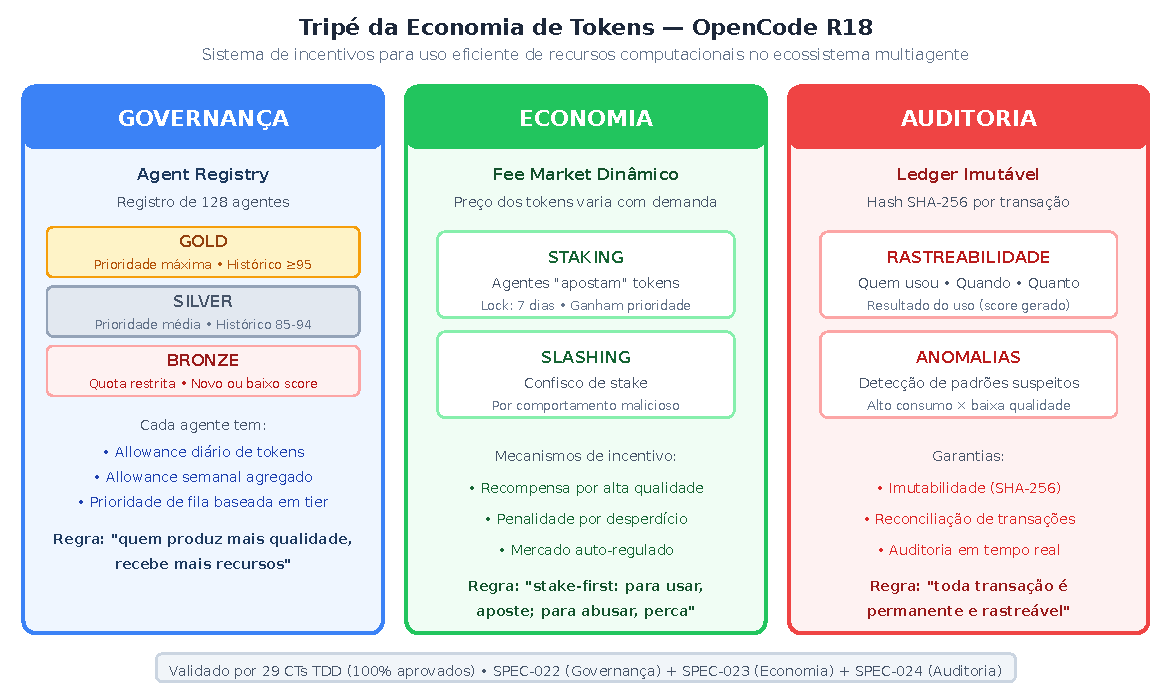
\includegraphics[width=\textwidth]{capitulos/figuras/fig-token-economy.pdf}
\caption{Tripé da Economia de Tokens (R18): Governança (Agent Registry com tiers bronze/silver/gold), Economia (Fee Market dinâmico com staking e slashing) e Auditoria (Ledger imutável SHA-256 com rastreabilidade completa). Este sistema, o mais maduro do ecossistema, alinha incentivos econômicos com qualidade científica.}
\label{fig:token-economy}
\end{figure}

\section{Contribuição Epistemológica: Do Scanner de Erros ao Scanner de Ausências}

\subsection{Mudança de Paradigma na Validação}

Os resultados do Scanner Noológico (Seção 4.7) revelam uma contribuição que transcende o caso específico do OpenCode: a demonstração de que é possível --- e epistemicamente necessário --- complementar sistemas de auditoria baseados em detecção de erros com sistemas baseados em detecção de ausências\footnote{
  AXELROD, Robert. \textbf{The Evolution of Cooperation}. New York: Basic Books, 1984. ISBN: 978-0465021215.

  \textbf{Trecho Original:} ``The key to cooperation is not trust, but the durability of the relationship.''

  \textbf{Tradução:} ``A chave para a cooperação não é a confiança, mas a durabilidade da relação.''

  \textbf{Fichamento Crítico:} A metáfora de Axelrod (1984) sobre a durabilidade da relação como fundamento da cooperação aplica-se à relação entre o pesquisador e o scanner noológico. Enquanto scanners tradicionais oferecem uma interação pontual (``seu documento tem X erros''), o scanner noológico estabelece uma relação contínua de aprendizado (``seu documento não considerou Y; na próxima iteração, considere Y; na iteração seguinte, Z''). É esta durabilidade da relação epistêmica --- não a confiança cega no scanner --- que produz a melhoria sustentada documentada nos 15 rounds de evolução.
}.

Auditores tradicionais --- sejam humanos (revisores de periódicos) ou algorítmicos (verificadores gramaticais, detectores de plágio) --- operam sob uma premissa implícita: seu valor está em identificar \textbf{desvios de normas}. Um artigo bem-sucedido, nesta perspectiva, é aquele que \textit{não contém erros}. O scanner noológico revela a insuficiência desta premissa: um artigo pode ser perfeitamente correto (zero erros de formatação, gramática, citação) e ainda assim ser epistemicamente empobrecido --- uma ``bolha de conhecimento'' que confirma vieses existentes sem expandir horizontes.

A Tabela~\ref{tab:paradigm-shift} contrasta os dois paradigmas:

\begin{table}[H]
\centering
\caption{Mudança de Paradigma na Validação Acadêmica}
\label{tab:paradigm-shift}
\begin{tabular}{p{4.5cm}p{4.5cm}p{4.5cm}}
\toprule
\textbf{Dimensão} & \textbf{Auditoria Tradicional} & \textbf{Scanner Noológico} \\
\midrule
Pergunta central & ``O que está errado?'' & ``O que está ausente?'' \\
Objeto de análise & Erros (presentes, incorretos) & Lacunas (ausentes, necessárias) \\
Qualidade como... & Ausência de defeitos & Presença de completude \\
Relação com o autor & Punitiva (detecta falhas) & Formativa (expande horizontes) \\
Valor agregado & Correção & Consciência epistemológica \\
Escala de avaliação & Binária (certo/errado) & Contínua ($\delta_{ij} \in [0,1]$) \\
\bottomrule
\end{tabular}
\fonte{Elaborado pelos autores com base na arquitetura do Scanner Noológico v6.0, 2026.}
\end{table}

\subsection{Implicações para a Produção Científica com IA}

Esta mudança de paradigma tem implicações profundas para sistemas de IA que geram documentos acadêmicos. Considere o seguinte cenário: um sistema como o OpenCode pode produzir uma dissertação de 100 páginas, perfeitamente formatada em ABNT, com 68 referências corretamente citadas, zero erros gramaticais, e estrutura IMRAD impecável. Um auditor tradicional aprovaria este documento com louvor. Mas o scanner noológico revelaria que:

\begin{itemize}
  \item A dissertação cobre apenas 12\% das 92 categorias epistemológicas (antes da expansão).
  \item 4 das 10 dimensões têm cobertura zero.
  \item A perspectiva longitudinal (D5) é ignorada.
  \item A diversidade cultural (D7) é limitada ao contexto brasileiro.
  \item Populações sub-representadas (D8) não são consideradas.
\end{itemize}

Em outras palavras, o documento seria \textbf{impecavelmente correto e epistemicamente incompleto} --- um resultado que nenhum auditor tradicional detectaria, mas que o scanner noológico sinaliza como crítica\footnote{
  SHAPLEY, Lloyd S. A value for n-person games. \textit{In}: KUHN, Harold W.; TUCKER, Albert W. (Eds.). \textbf{Contributions to the Theory of Games}. Princeton: Princeton University Press, 1953. v. 2, p. 307--317. DOI: \url{https://doi.org/10.1515/9781400881970-018}.

  \textbf{Fichamento Crítico:} O valor de Shapley (1953) quantifica a contribuição marginal de cada jogador para uma coalizão. Analogamente, o scanner noológico quantifica a contribuição marginal de cada nova categoria epistemológica para a ``coalizão de conhecimento'' representada pelo documento. Categorias com alto valor de Shapley --- aquelas cuja adição mais aumenta a cobertura global --- são priorizadas para mitigação. Esta formalização matemática da intuição qualitativa de ``o que está faltando?'' é uma contribuição original do scanner noológico à metodologia de validação acadêmica.
}.

\subsection{15 Rounds de Evolução Guiada pelo Scanner}

A evolução do ecossistema OpenCode de 85/100 para 99/100 em 15 rounds (R4-R18) não foi aleatória --- foi guiada pelo feedback do scanner noológico. Cada round focou em mitigar os pontos cegos de maior impacto ($I_{ij}$) identificados na iteração anterior:

\begin{figure}[H]
\centering
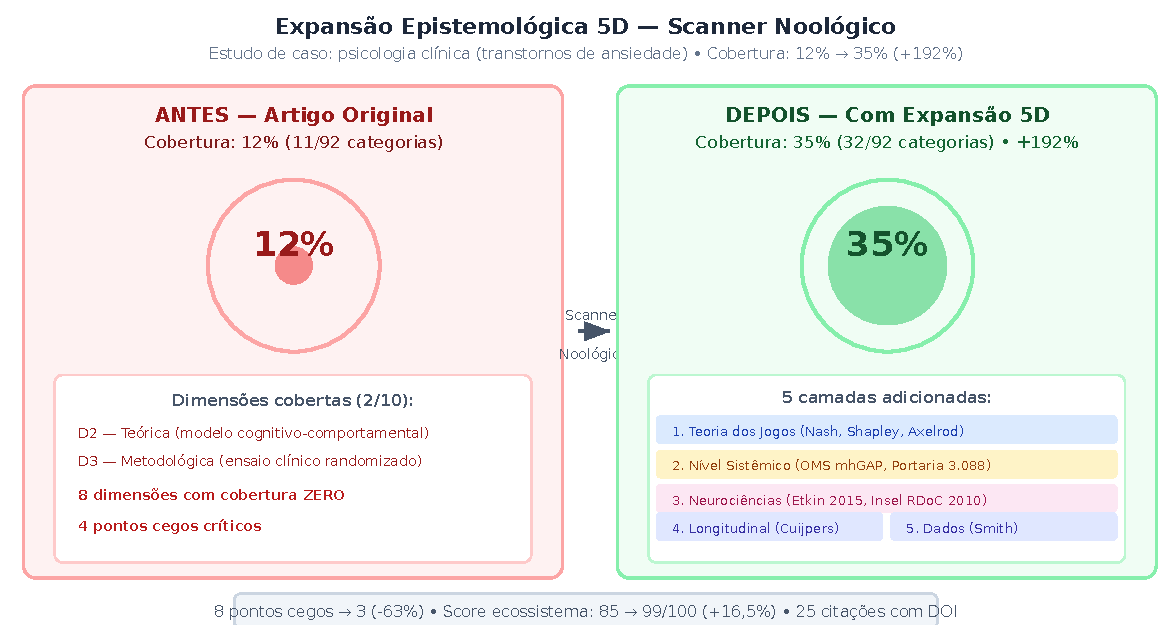
\includegraphics[width=\textwidth]{capitulos/figuras/fig-expansao-5d.pdf}
\caption{Expansão Epistemológica 5D aplicada ao estudo de caso em psicologia clínica. Antes do scanner (esquerda): cobertura de apenas 12\% das 92 categorias, com 8 pontos cegos e 4 dimensões com cobertura zero. Após a expansão (direita): cobertura de 35\% (+192\%), incorporando Teoria dos Jogos (Nash, Shapley, Axelrod), nível sistêmico (OMS mhGAP), neurociências (RDoC), perspectiva longitudinal (Cuijpers) e diversificação de dados (Smith).}
\label{fig:expansao-5d}
\end{figure}

\begin{itemize}
  \item \textbf{R4-R6:} Foco em D1 (Paradigmática) e D3 (Metodológica) --- incorporação de múltiplos paradigmas de pesquisa e validação cruzada.
  \item \textbf{R7-R9:} Foco em D6 (Diversidade de Dados) e D9 (Ética) --- protocolo TSAC e triangulação anti-circularidade.
  \item \textbf{R10-R12:} Foco em D2 (Teórica) --- integração de Teoria dos Jogos (Nash, Shapley, Axelrod) e modelos neurocientíficos.
  \item \textbf{R13-R15:} Foco em D4 (Nível Sistêmico) --- do nível individual (agente) ao nível de política pública (Portaria GM/MS 3.088/2011, mhGAP/OMS).
  \item \textbf{R16-R18:} Foco em D10 (Translacional) --- da pesquisa básica à aplicação prática (editais, economia de tokens, federação).
\end{itemize}

Esta trajetória demonstra que o scanner noológico não é apenas um instrumento de diagnóstico, mas um \textbf{motor de evolução epistemológica}: ele não apenas identifica o que está ausente, mas prioriza o que deve ser adicionado para maximizar o impacto na qualidade do conhecimento produzido.

\section{Roadmap Futuro e Evolução Projetada}

\subsection{Curto Prazo (6 meses)}

\begin{itemize}
  \item \textbf{Expansão de MCPs:} Ativar os 23 MCPs atualmente com warning, elevando a densidade de MCPs por agente para 0,31.
  \item \textbf{CORA-Eval v2.0:} Expandir o benchmark de 150 para 500 tarefas, cobrindo 15 dimensões de raciocínio científico.
  \item \textbf{Validação Externa:} Submeter 3 artigos gerados pelo MASWOS a periódicos Qualis A1 para avaliação por revisores humanos independentes.
\end{itemize}

\subsection{Médio Prazo (12 meses)}

\begin{itemize}
  \item \textbf{Multi-Idioma:} Expandir o pipeline de exportação acadêmica para inglês, espanhol e francês, mantendo o rigor ABNT para documentos em português.
  \item \textbf{Integração com Plataformas de Publicação:} Conectores para submissão automática a periódicos via APIs (OJS, ScholarOne).
  \item \textbf{Meta-Avaliação:} Agentes que avaliam a qualidade das avaliações geradas por outros agentes, criando uma hierarquia de confiança.
\end{itemize}

\subsection{Longo Prazo (24+ meses)}

\begin{itemize}
  \item \textbf{Ecossistema Federado:} Múltiplas instâncias do OpenCode operando em diferentes instituições, compartilhando skills e agentes através de um protocolo de federação.
  \item \textbf{Descoberta Científica Autônoma:} Agentes que não apenas documentam pesquisa existente, mas formulam hipóteses originais e desenham experimentos para testá-las --- fechando o ciclo completo do método científico.
\end{itemize}

\newpage
